\subsection{Introduction}
AlphaGo is a groundbreaking AI model that utilizes neural networks and tree
search to play the game of Go, which is thought to be one of the most
challenging classic games for artificial intelligence owing to its enormous
search space and the difficulty of evaluating board positions and moves
\cite{Silver2016}. \\\\ AlphaGo uses value networks for position evaluation and
policy networks for taking actions, that combined with Monte Carlo simulation
achieved a 99.8\% winning rate, and beating the European human Go champion in 5
out 5 games.

\subsection{Key Innovations}

\subsubsection*{Integration of Policy and Value Networks with MCTS}
AlphaGo combines policy and value networks in an MCTS framework to efficiently explore and evaluate the game tree. Each edge \( (s, a) \) in the search tree stores:
\begin{itemize}
    \item Action value \( Q(s, a) \): The average reward for taking action \( a \) from
          state \( s \).
    \item Visit count \( N(s, a) \): The number of times this action has been explored.
    \item Prior probability \( P(s, a) \): The probability of selecting action \( a \),
          provided by the policy network.
\end{itemize}

During the selection phase, actions are chosen to maximize:
\begin{equation}
    a_t = \arg\max_a \left( Q(s, a) + u(s, a) \right)
\end{equation}

where the exploration bonus \( u(s, a) \) is defined as:
\begin{equation}
    u(s, a) \propto \frac{P(s, a)}{1 + N(s, a)}
\end{equation}

When a simulation reaches a leaf node, its value is evaluated in two ways: 1.
Value Network Evaluation: A forward pass through the value network predicts \(
v_\theta(s) \), the likelihood of winning. 2. Rollout Evaluation: A lightweight
policy simulates the game to its conclusion, and the terminal result \( z \) is
recorded.

These evaluations are combined using a mixing parameter \( \lambda \):
\begin{equation}
    V(s_L) = \lambda v_\theta(s_L) + (1 - \lambda) z_L
\end{equation}

The back propagation step updates the statistics of all nodes along the path
from the root to the leaf. \\\\ It's also worth noting that the SL policy
network performed better than the RL policy network and that's probably because
humans select a diverse beam of promising moves, whereas RL optimizes for the
single best move.

Conversely though, the value network that was derived from the RL policy
performed better than the one derived from the SL policy.
\begin{figure}[htbp]
    \centering
    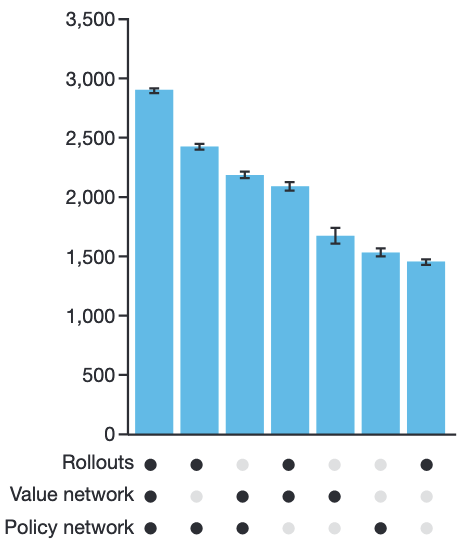
\includegraphics[width=0.9\linewidth, keepaspectratio]{sections/4AlphaGo/innovation.png}
    \caption{Performance of AlphaGo, on a single machine, for different
combinations of components.}
\end{figure}

\subsection{Training Process}

\subsubsection{Supervised Learning for Policy Networks}
The policy network was initially trained using supervised learning on human
expert games. The training data consisted of 30 million board positions sampled
from professional games on the KGS Go Server. The goal was to maximize the
likelihood of selecting the human move for each position:
\begin{equation}
    \Delta \sigma \propto \nabla_\sigma \log p_\sigma(a | s)
\end{equation}

where \( p_\sigma(a | s) \) is the probability of selecting action \( a \)
given state \( s \).

This supervised learning approach achieved a move prediction accuracy of 57.0\%
on the test set, significantly outperforming prior methods. This stage provided
a solid foundation for replicating human expertise.

\subsubsection{Reinforcement Learning for Policy Networks}
The supervised learning network was further refined through reinforcement
learning (RL). The weights of the RL policy network were initialized from the
SL network. AlphaGo then engaged in self-play, where the RL policy network
played against earlier versions of itself to iteratively improve.

The reward function used for RL was defined as:
\begin{equation}
    r(s) =
    \begin{cases}
        +1 & \text{if win}                           \\
        -1 & \text{if loss}                          \\
        0  & \text{otherwise (non-terminal states).}
    \end{cases}
\end{equation}

At each time step \( t \), the network updated its weights to maximize the
expected reward using the policy gradient method:
\begin{equation}
    \Delta \rho \propto z_t \nabla_\rho \log p_\rho(a_t | s_t)
\end{equation}

where \( z_t \) is the final game outcome from the perspective of the current
player.

This self-play strategy allowed AlphaGo to discover novel strategies beyond
human knowledge. The RL policy network outperformed the SL network with an 80\%
win rate and achieved an 85\% win rate against Pachi, a strong open-source Go
program, without using MCTS.

\subsubsection{Value Network Training}
The value network was designed to evaluate board positions by predicting the
likelihood of winning from a given state. Unlike the policy network, it outputs
a single scalar value \( v_\theta(s) \) between \(-1\) (loss) and \(+1\) (win).

Training the value network on full games led to overfitting due to the strong
correlation between successive positions in the same game. To mitigate this, a
new dataset of 30 million distinct board positions was generated through
self-play, ensuring that positions came from diverse contexts.

The value network was trained by minimizing the mean squared error (MSE)
between its predictions \( v_\theta(s) \) and the actual game outcomes \( z \):
\begin{equation}
    L(\theta) = \mathbb{E}_{(s, z) \sim D} \left[ (v_\theta(s) - z)^2 \right]
\end{equation}

\begin{figure}[htbp]
    \centering
    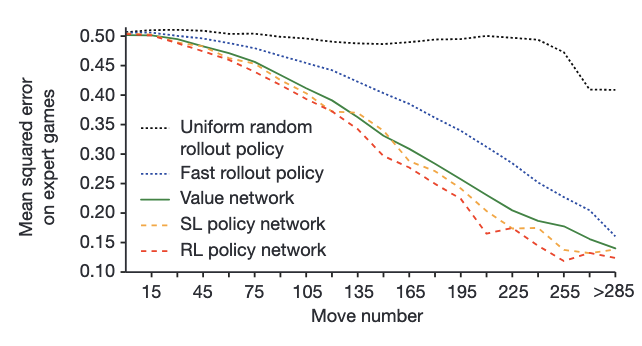
\includegraphics[width=\linewidth, keepaspectratio]{sections/4AlphaGo/mse.png}
    \caption{Comparison of evaluation
accuracy between the value network and rollouts with different policies.}
\end{figure}

\subsection{Challenges and Solutions}
AlphaGo overcame several challenges:
\begin{itemize}
    \item Overfitting: Training the value network on full games led to memorization. This
          was mitigated by generating a diverse self-play dataset.
    \item Scalability: Combining neural networks with MCTS required significant
          computational resources, addressed through parallel processing on GPUs and
          CPUs.
    \item Exploration vs. Exploitation: Balancing these in MCTS was achieved using the
          exploration bonus \( u(s, a) \) and the policy network priors.
\end{itemize}

\subsection{Performance Benchmarks}
AlphaGo achieved the following milestones:
\begin{itemize}
    \item 85\% win rate against Pachi without using MCTS.
    \item 99.8\% win rate against other Go programs in a tournament held to evaluate the performance of AlphaGo.
    \item Won 77\%, 86\%, and 99\% of handicap games against Crazy Stone, Zen and Pachi,
          respectively.
    \item Victory against professional human players such as Fan Hui (5-0) and Lee Sedol
          (4-1), marking a significant breakthrough in AI.
\end{itemize}

\begin{figure}[htbp]
    \centering
    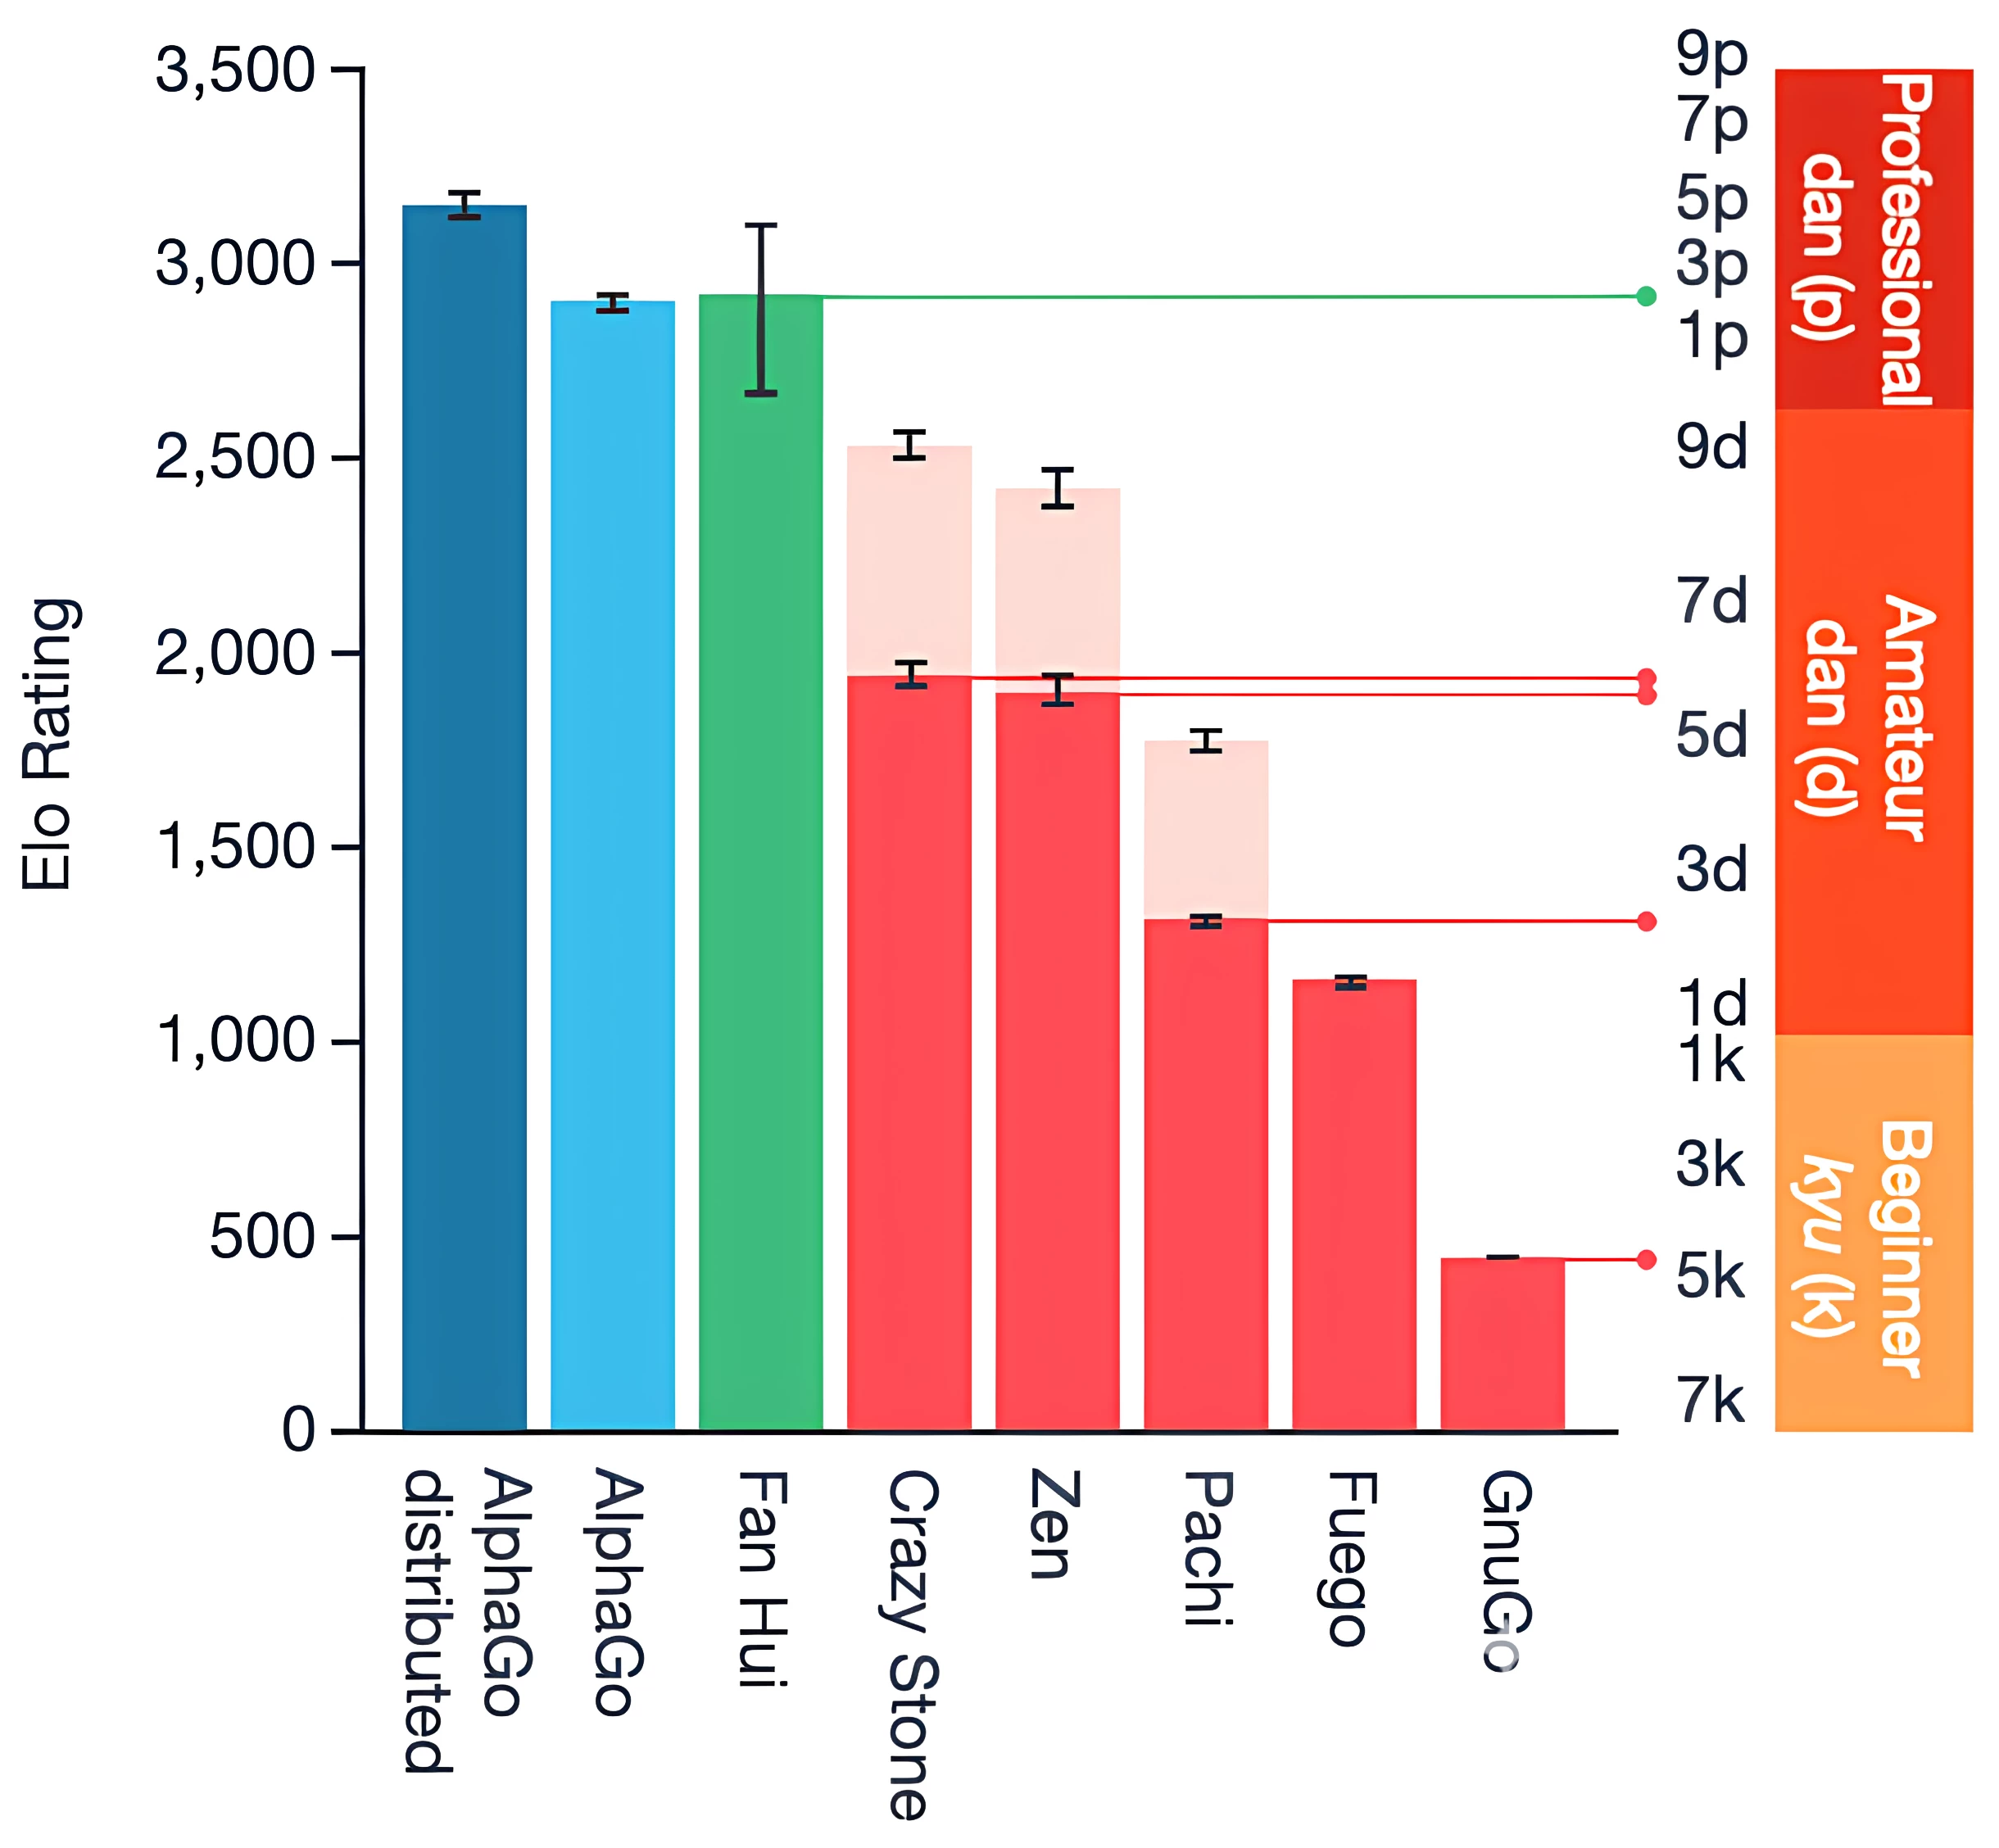
\includegraphics[width=\linewidth, keepaspectratio]{sections/4AlphaGo/comparison.png}
    \caption{Elo rating comparison between AlphaGo and other Go programs.}
\end{figure}
